% Figure 1 of article/main_layout.tex: the DeCovarT pipeline applied to the
% Suppinger gastruloids, on one portrait A4 page (210 x 297 mm).
% Layout after scConcept Fig. 1 (Bahrami et al., bioRxiv 2025, p. 4): the main
% steps on a grey trunk on the left, the details in dashed panels on the right,
% each step joined to its panel by a grey gradient wedge.
%
% The ggplot2 panels and values.tex come from article/scripts/fig01_pipeline.R.
% Build, from the DeCovarT repository root:
%   Rscript --no-save --no-restore article/scripts/fig01_pipeline.R
%   cd article/scripts && latexmk -lualatex -outdir=../figs fig01_pipeline.tex
%   latexmk -c -outdir=../figs fig01_pipeline.tex
%   cd ../figs && pdftocairo -svg fig01_pipeline.pdf fig01_pipeline.svg
% Sources of the content:
%   a  DeCovarT_reproducibility/docs/02-feature-selection.qmd (tiers i-ii),
%      vignettes/03-1-feature-selection.qmd (fig-fs-tiers)
%   b  DeCovarT_reproducibility/docs/03-covariance-estimation.qmd,
%      docs/04-deconvolution-pipeline.qmd (sec-deconv-selection)
%   c  vignettes/05-1-review-distribution-aware.qmd (fig-ladder),
%      review-decovart-bastien-elias-marielle-anais/answer_elias.qmd (selected model)
%   d  DeCovarT_reproducibility/docs/05-biological-insights.qmd
\documentclass[border=0pt]{standalone}
\usepackage{iftex}
\ifPDFTeX
  \PackageError{fig01}{Use LuaLaTeX}{}
\fi
\usepackage{fontspec}
\setmainfont{Noto Sans}
\usepackage{amsmath,amssymb,bm}
\usepackage{graphicx}
\usepackage{xcolor}
\usepackage{tikz}
\usetikzlibrary{bayesnet,arrows.meta,positioning,fit,calc,backgrounds,shapes.geometric}
% Written by article/scripts/fig01_pipeline.R; do not edit by hand.
% Colours: data/dictionaries/suppinger_celltype_colours.csv (reproducibility repository).
\definecolor{ctEctopic}{HTML}{D899BA}
\definecolor{ctNaive}{HTML}{8C0062}
\definecolor{ctEpiblast}{HTML}{6D3C00}
\definecolor{ctStreak}{HTML}{C9A580}
\definecolor{ctCaudal}{HTML}{005D22}
\definecolor{ctPSM}{HTML}{006F3B}
\definecolor{ctSomite}{HTML}{00936A}
\definecolor{ctGut}{HTML}{8FAED5}
\newcommand{\nDeposited}{27,027}
\newcommand{\nPresence}{9,633 / 10,751 / 9,761}
\newcommand{\nWelch}{1,360 / 3,617 / 5,893}
\newcommand{\nUnion}{6,749}
\newcommand{\nGenesD}{5,821}

\graphicspath{{../figs/fig01_pipeline/}}

% scalecol, fixedpar and eqnote repeat article/macros.tex (that file also
% defines \strong, which clashes here, so it is not \input).
\definecolor{scalecol}{HTML}{C45C26}
\definecolor{ink}{HTML}{1C2B24}
\definecolor{series}{HTML}{1D4E89}
\definecolor{accent}{HTML}{C45C26}
\definecolor{trunk}{HTML}{EEEDEA}
\definecolor{trunkdraw}{HTML}{B9B4AA}
\definecolor{latfill}{HTML}{DAE9FB}
\definecolor{latdraw}{HTML}{4477B5}
\definecolor{gastrolight}{HTML}{C9D5E0}
\definecolor{gastrodark}{HTML}{5F7F99}

\hyphenpenalty=10000
\exhyphenpenalty=10000

\newcommand{\bmu}{\tilde{\boldsymbol{\mu}}}
\newcommand{\SigW}{\hat{\boldsymbol{\Sigma}}_{W,j}}

\tikzset{
  every node/.style={text=ink},
  fixedpar/.style={const, draw, minimum size=16pt, inner sep=2pt, font=\small},
  eqnote/.style={font=\scriptsize, align=center, inner sep=1pt},
  stepbox/.style={draw=trunkdraw, fill=white, rounded corners=3pt, line width=0.6pt},
  steptitle/.style={font=\bfseries\small, anchor=north west, inner sep=0pt},
  panel/.style={draw=ink!55, dashed, rounded corners=4pt, line width=0.5pt, fill=white},
  paneltitle/.style={font=\bfseries\footnotesize, anchor=north west, inner sep=0pt, text width=108mm},
  letter/.style={font=\bfseries\large, anchor=north west, inner sep=0pt},
  small/.style={font=\scriptsize, align=center, inner sep=1pt},
  flow/.style={-{Stealth[length=2.2mm]}, line width=0.8pt, draw=ink!70},
  thin/.style={-{Stealth[length=1.6mm]}, line width=0.5pt, draw=ink!70},
  wnt/.style={-{Stealth[length=1.5mm]}, line width=0.7pt},
  % gradient wedge from a step (narrow, left) to its panel (wide, right)
  wedge/.style={left color=black!22, right color=white, draw=none},
}

% \wedge{x0}{y0 bottom}{y0 top}{x1}{y1 bottom}{y1 top}
\newcommand{\wedgeshape}[6]{%
  \shade[wedge] (#1,#2) -- (#4,#5) -- (#4,#6) -- (#1,#3) -- cycle;}

% A gastruloid stage of the timeline: a disc of radius #3 at (#1,#2)
\newcommand{\blob}[3]{%
  \shade[inner color=gastrolight, outer color=gastrodark, draw=gastrodark!80!black, line width=0.3pt]
    (#1,#2) circle (#3);}

% Wnt pulse: a short zigzag arrow ending at (#1,#2), colour #3
\newcommand{\wntpulse}[3]{%
  \draw[wnt, draw=#3] ($(#1,#2)+(0.6,6.2)$) -- ++(-1.2,-2) -- ++(1.4,-0.4) -- ++(-0.8,-2.3);}

\begin{document}
\begin{tikzpicture}[x=1mm, y=1mm]
\useasboundingbox (0,0) rectangle (210,297);

% ===================== left trunk ==========================================
\fill[trunk, rounded corners=6pt] (8,8) rectangle (72,289);
\node[font=\bfseries\small, anchor=north, text=ink!80] at (40,287.5) {DeCovarT pipeline};

% step boxes: A 226-278, B 157-201, C 81-137, D 13-63
\coordinate (A-b) at (12,226); \coordinate (A-t) at (68,278);
\coordinate (B-b) at (12,157); \coordinate (B-t) at (68,201);
\coordinate (C-b) at (12,81);  \coordinate (C-t) at (68,137);
\coordinate (D-b) at (12,13);  \coordinate (D-t) at (68,63);

% gradient wedges (drawn first, under the boxes and panels)
\wedgeshape{68}{226}{278}{84}{213}{289}
\wedgeshape{68}{157}{201}{84}{149}{209}
\wedgeshape{68}{100.5}{109.5}{84}{73}{145}
\wedgeshape{68}{13}{63}{84}{8}{69}

\foreach \s in {A,B,C,D} {\draw[stepbox] (\s-b) rectangle (\s-t);}
\draw[flow] (40,226) -- (40,201);
\draw[flow] (40,157) -- (40,137);
\draw[flow] (40,81) -- (40,63);

% ---- A step: gene selection funnel ----------------------------------------
\node[letter] at (13.5,276.5) {a};
\node[steptitle] at (19,276.5) {Gene selection};
\begin{scope}
  \fill[series!25] (18,265) -- (62,265) -- (56,257) -- (24,257) -- cycle;
  \fill[series!50] (24,256) -- (56,256) -- (51,248) -- (29,248) -- cycle;
  \fill[series!75] (29,247) -- (51,247) -- (47,239) -- (33,239) -- cycle;
  \fill[accent] (33,238) -- (47,238) -- (45,232) -- (35,232) -- cycle;
  \node[small] at (40,261) {\nDeposited\ genes};
  \node[small] at (40,252) {(1) presence};
  \node[small, text=white] at (40,243) {(2) Welch $G$};
  \node[small, text=white] at (40,235) {(3) BH};
  \node[small, anchor=west] at (48.5,235) {\nUnion};
\end{scope}

% ---- B step: reference moments and scale-free bulk likelihood -------------
\node[letter] at (13.5,199.5) {b};
\node[steptitle] at (19,199.5) {Reference moments};
\node[small, anchor=north west, text width=50mm, align=left] at (15,193)
  {cells of type $j$ $\;\longrightarrow\;$ mean $\bmu_{\cdot j}$,\\[1pt]
   shrunk covariance $\SigW(\lambda)$};
\draw[thin] (40,180) -- (40,175);
\node[small, anchor=north west, text width=50mm, align=left] at (15,173)
  {bulk likelihood with free scales\\[1pt]
   $\lambda$ chosen on the bulk replicates};

% ---- C step: ladder of noise models ---------------------------------------
\node[letter] at (13.5,135.5) {c};
\node[steptitle] at (19,135.5) {Noise model of the bulk};
\begin{scope}
  \def\ladderlabels{{"OLS / NNLS","weighted LS","mean--variance GLM","variance linear in $\boldsymbol{p}$","GLS, dense $G\times G$","sandwich / GEE","GLMM"}}
  \draw[ink, line width=1.1pt] (16,83) -- (16,129);
  \draw[ink, line width=1.1pt] (26,83) -- (26,129);
  \foreach \k in {1,...,7} {
    \pgfmathsetmacro{\yy}{80+6*\k}
    \pgfmathsetmacro{\lab}{\ladderlabels[\k-1]}
    \ifnum\k=4
      \fill[latfill, draw=latdraw, line width=0.6pt, rounded corners=1.5pt] (14.5,\yy-2.6) rectangle (67,\yy+2.6);
    \fi
    \draw[ink, line width=0.8pt] (16,\yy) -- (26,\yy);
    \node[font=\scriptsize, anchor=west, inner sep=0pt] at (28,\yy) {\k\enspace\lab};
  }
\end{scope}

% ---- D step: gastruloid timeline, two Wnt timings -------------------------
\node[letter] at (13.5,61.5) {d};
\node[steptitle] at (19,61.5) {Gastruloids: Wnt timing};
\begin{scope}
  \foreach \t/\x in {0/17,24/27,48/37,72/47,96/60} {
    \node[font=\tiny, inner sep=0pt] at (\x,16.5) {\t\,h};
  }
  \draw[ink!40, line width=0.4pt] (14,19) -- (66,19);
  % standard row: pulse at 48 h, elongated trunk at 96 h
  \node[font=\scriptsize, anchor=west, text=series] at (14,53.5) {standard};
  \foreach \dx/\dy in {0/0,1.1/0.4,0.5/-0.9,-0.8/0.6,-0.4/-0.7} {\fill[gastrodark] (17+\dx,45+\dy) circle (0.35);}
  \blob{27}{45}{1.8}
  \blob{37}{45}{2.6}
  \blob{47}{45}{3.2}
  \wntpulse{37}{48.2}{series}
  \shade[left color=ctPSM!45, right color=ctCaudal!80, draw=ctPSM!70!black, line width=0.3pt]
    plot[smooth cycle, tension=0.8] coordinates {(54,44) (56,47.4) (60,48.4) (65,47.6) (66.4,45) (64.5,42.8) (60,43.3) (56,42.2)};
  % early row: pulse at 24 h, ovoid with a pluripotent core at 96 h
  \node[font=\scriptsize, anchor=west, text=accent] at (14,36.5) {early};
  \foreach \dx/\dy in {0/0,1.1/0.4,0.5/-0.9,-0.8/0.6,-0.4/-0.7} {\fill[gastrodark] (17+\dx,28+\dy) circle (0.35);}
  \blob{27}{28}{1.8}
  \blob{37}{28}{2.6}
  \blob{47}{28}{3.2}
  \wntpulse{27}{30.9}{accent}
  \shade[inner color=ctPSM!35, outer color=ctCaudal!70, draw=ctPSM!70!black, line width=0.3pt]
    plot[smooth cycle, tension=0.9] coordinates {(55.5,28) (57,31.6) (61,32.6) (64.6,30.6) (65,26.6) (61.6,24.2) (57,24.6)};
  \fill[ctEctopic!85] plot[smooth cycle, tension=0.9] coordinates {(57.8,28.4) (59.4,30.8) (62,30.4) (62.6,27.4) (60.4,26)};
  \foreach \y in {45,28} {\draw[thin, ink!45] (50.6,\y) -- (53.4,\y);}
  \node[font=\tiny, text=series] at (37,55.8) {Wnt};
  \node[font=\tiny, text=accent] at (27,38.5) {Wnt};
\end{scope}

% ===================== right panels ========================================
\draw[panel] (84,213) rectangle (202,289);
\draw[panel] (84,149) rectangle (202,209);
\draw[panel] (84,73) rectangle (202,145);
\draw[panel] (84,8) rectangle (202,69);

% ---- A panel: three gates, then the gene counts ---------------------------
\node[paneltitle] at (88,287) {Three gates, applied at 48, 72 and 96 h on the single-cell reference};
\foreach \x/\lab in {88/{(1) present in every type}, 126/{(2) permuted Welch $G$}, 164/{(3) Benjamini--Hochberg}} {
  \node[font=\scriptsize\bfseries, anchor=south west, inner sep=0pt] at (\x,278.6) {\lab};
}
\node[anchor=south west, inner sep=0pt] at (88,254) {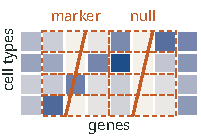
\includegraphics{panel_a1_presence.pdf}};
\node[anchor=south west, inner sep=0pt] at (126,254) {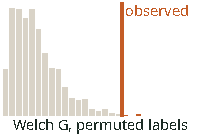
\includegraphics{panel_a2_welch.pdf}};
\node[anchor=south west, inner sep=0pt] at (164,254) {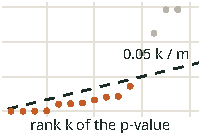
\includegraphics{panel_a3_bh.pdf}};
\draw[flow] (122.3,265.5) -- (125.7,265.5);
\draw[flow] (160.3,265.5) -- (163.7,265.5);
\node[small, anchor=north west, align=left, text width=36mm] at (88,253.5)
  {$\ge 20$ cells; $\ge 2$ cells and variance $>0$ in every type: drops markers and null genes};
\node[small, anchor=north west, align=left, text width=36mm] at (126,253.5)
  {type effect, $B=2000$ label permutations;\\ $p=(1+\#\{G^{*}\ge G\})/(B+1)$};
\node[small, anchor=north west, align=left, text width=36mm] at (164,253.5)
  {false discovery rate at $0.05$ over the genes tested};
\node[anchor=south west, inner sep=0pt] at (88,214.5) {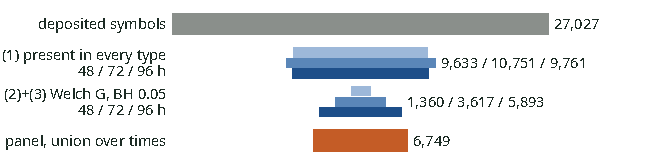
\includegraphics{panel_a4_funnel.pdf}};

% ---- B panel: shrinkage and the scale-free bulk likelihood ----------------
\node[paneltitle] at (88,206.5) {Covariance shrunk toward its diagonal, level chosen on the bulk};
\node[small, anchor=north west, align=left] at (88,200)
  {$\SigW(\lambda)=\boldsymbol{\Delta}_j^{1/2}\{(1-\lambda)\boldsymbol{R}_j+\lambda\mathbf{I}\}\boldsymbol{\Delta}_j^{1/2}$};
\node[anchor=south west, inner sep=0pt] at (87,169) {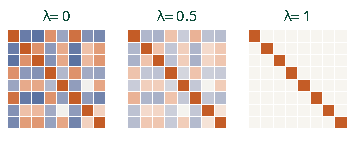
\includegraphics{panel_b1_shrinkage.pdf}};
\node[small, anchor=north west, align=left, text width=60mm] at (88,167.5)
  {$\boldsymbol{m}_i=c_i\,\bmu\,\boldsymbol{p}_{\cdot i}$,\quad
   $\boldsymbol{\Sigma}_i=\phi_i\textstyle\sum_j p_{ji}\SigW(\lambda)$\\[2pt]
   mean scale $c_i=a_in_i$ and variance scale $\phi_i=a_i^{2}n_i$ profiled out in closed form: no cell count or library size is needed};
\node[anchor=south west, inner sep=0pt] at (150,165) {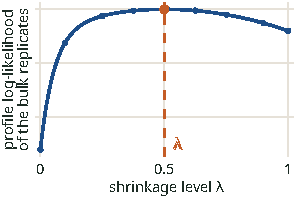
\includegraphics{panel_b2_loglik.pdf}};
\node[small, anchor=north west, align=left, text width=50mm] at (150,163)
  {$\hat\lambda$ maximises the profile likelihood summed over the three bulk replicates; the composition is never read (curve symbolic)};

% ---- C panel: selected DeCovarT model -------------------------------------
\node[paneltitle] at (88,142.5) {Selected model: a bulk is a sum of independent cells};
\begin{scope}[every node/.append style={font=\small}]
  % reference side
  \node[obs] (x) at (99,111) {$\boldsymbol{x}_{\cdot c}$};
  \plate[inner sep=2.2mm]{cells}{(x)}{$c=1,\ldots,C_j$};
  \node[det] (mu) at (124,122) {$\bmu_{\cdot j}$};
  \node[det] (sw) at (124,100) {$\SigW$};
  \node[eqnote, font=\scriptsize, anchor=west] (nsw) at (90.5,89) {$\boldsymbol{\Delta}_j^{1/2}\{(1-\lambda)\boldsymbol{R}_j+\lambda\mathbf{I}\}\boldsymbol{\Delta}_j^{1/2}$};
  \draw[->] (cells) -- (mu);
  \draw[->] (cells) -- (sw);
  \plate[inner sep=2.2mm]{types}{(cells)(cells-caption)(mu)(sw)(nsw)}{$j=1,\ldots,J$};
  \node[fixedpar] (lam) at (139.5,88) {$\lambda$};
  \draw[->] (lam) -- (sw);
  % bulk side
  \node[fixedpar] (p) at (153,132) {$\boldsymbol{p}_{\cdot i}$};
  \node[fixedpar, draw=scalecol] (a) at (167,132) {$a_i$};
  \node[fixedpar, draw=scalecol] (n) at (181,132) {$n_i$};
  \node[det] (m) at (158,116) {$\boldsymbol{m}_i$};
  \node[det] (S) at (158,100) {$\boldsymbol{\Sigma}_i$};
  \node[obs] (y) at (185,108) {$\boldsymbol{y}_{\cdot i}$};
  \node[eqnote, font=\scriptsize, align=left, anchor=north west] (nb) at (147,91)
    {$\boldsymbol{y}_{\cdot i}\sim\mathcal{N}_G(\boldsymbol{m}_i,\boldsymbol{\Sigma}_i)$\\[1pt]
     $\boldsymbol{m}_i=a_in_i\,\bmu\,\boldsymbol{p}_{\cdot i}$\\[1pt]
     $\boldsymbol{\Sigma}_i=a_i^{2}n_i\sum_j p_{ji}\SigW$};
  \foreach \s in {p,a,n} {\draw[->] (\s) -- (m); \draw[->] (\s) -- (S);}
  \draw[->] (mu) -- (m);
  \draw[->] (sw) -- (S);
  \draw[->] (m) -- (y);
  \draw[->] (S) -- (y);
  \plate[inner sep=2.2mm]{bulk}{(p)(a)(n)(m)(S)(y)(nb)}{$i=1,\ldots,N$};
\end{scope}
\node[small, anchor=south west, align=left] at (88,74.2)
  {grey circle: observed;\enspace diamond: computed;\enspace square: fixed or estimated};

% ---- D panel: standard against early Wnt at 96 h --------------------------
\node[paneltitle] at (88,66.5) {96 h gastruloids: compositions estimated by DeCovarT};
% regular, trunk-like gastruloid above the standard facet
\begin{scope}[shift={(139,53)}, scale=0.92]
  \shade[left color=ctPSM!40, right color=ctCaudal!85, draw=ctPSM!70!black, line width=0.4pt]
    plot[smooth cycle, tension=0.75] coordinates {(-17,-1.5) (-14,3.6) (-6,6) (4,6.2) (12,5) (17.5,1.8) (18,-2.4) (13,-5) (4,-4.8) (-6,-5.6) (-14,-5.2)};
  \draw[ctGut, line width=1.2pt, line cap=round] plot[smooth, tension=0.7] coordinates {(-12,-0.6) (-4,0.6) (5,0.2) (12,-0.4)};
  \foreach \x in {-13,-9.6,-6.2} {\draw[ctSomite!80!black, line width=0.4pt, fill=ctSomite!40] (\x,3.0) circle (1.1); \draw[ctSomite!80!black, line width=0.4pt, fill=ctSomite!40] (\x,-3.6) circle (1.1);}
  \node[font=\scriptsize, text=series, anchor=north] at (0,-6.8) {elongated, trunk-like};
\end{scope}
% degenerate gastruloid above the early facet
\begin{scope}[shift={(179,53)}, scale=0.92]
  \shade[inner color=ctPSM!30, outer color=ctCaudal!75, draw=ctPSM!70!black, line width=0.4pt]
    plot[smooth cycle, tension=0.9] coordinates {(-12,0) (-9,5.4) (0,7) (9,5.6) (12.4,0.4) (9,-5.4) (0,-6.6) (-9,-5.2)};
  \fill[ctEctopic!85, draw=ctEctopic!70!black, line width=0.3pt]
    plot[smooth cycle, tension=0.9] coordinates {(-7,0.6) (-4.6,4.4) (1.4,4.8) (5.6,2) (5,-2.8) (0.4,-4.4) (-5,-3)};
  \draw[ctGut, line width=1.0pt, line cap=round] plot[smooth, tension=0.7] coordinates {(6.4,3.4) (8.6,0.4) (7.4,-3)};
  \node[font=\scriptsize, text=ink, align=center] at (-0.6,0.2) {ectopic\\[-2pt]pluripotency};
  \node[font=\scriptsize, text=accent, anchor=north] at (0,-6.8) {ovoid, no trunk};
\end{scope}
\node[small, anchor=north west, align=left, text width=29mm] at (88,62)
  {Early Wnt: ectopic pluripotency up, pre-somitic mesoderm down.\\[2pt]
   Shrinkage, $\hat\lambda$ on the bulk, \nGenesD\ genes.\\[2pt]
   $\Diamond$\,: single-cell reference, standard protocol.};
\node[anchor=south west, inner sep=0pt] at (88,9.5) {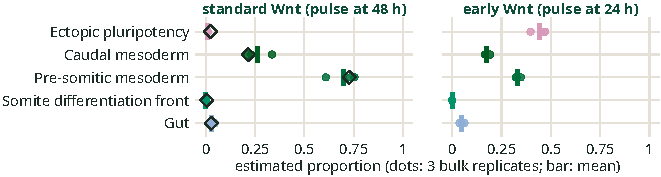
\includegraphics{panel_d_composition.pdf}};

\end{tikzpicture}
\end{document}
